%!TEX program = xelatex
%!BIB program = bibtex
\documentclass[cn,black,12pt,normal]{elegantnote}
\usepackage{float}
\usepackage{hyperref}
\usepackage{amsmath}
\usepackage{amsfonts}
\usepackage{amssymb}
\usepackage{siunitx}[=v2]
\usepackage{fancyhdr}
\usepackage{newtxtext}
\usepackage{algorithm}
\usepackage{algorithmic}
\newcommand{\uct}[1]{\textsuperscript{\textsuperscript{\cite{#1}}}}
\renewcommand{\tablename}{\textbf{Table}}
\renewcommand{\figurename}{Figure.}
\renewcommand{\refname}{References}
\renewcommand{\contentsname}{Contents}
\renewcommand{\versiontext}{Version: }
\renewcommand{\updatetext}{Update: }
\PassOptionsToPackage{no-math}{fontspec}
\lstset{basicstyle=\footnotesize\ttfamily\color[RGB]{50,0,130},numbers=none,frame=trBL}

\sisetup{mode=text}
\sisetup{range-phrase = \text{ \textasciitilde }}
\pagestyle{fancy}
\fancyhead[L]{School of Software Engineering, Tongji University}
\fancyhead[R]{Data Structure Projects}
\renewcommand{\headrulewidth}{1pt}

\title{Electrical grid\\电网建设造价模拟系统}
\author{1951510\; 姜文渊}
\institute{\small \url{https://github.com/jwyjohn/Jwy_DataStructureHomework}}
\version{0.50}
\date{\today}

\begin{document}

\maketitle

\section{Introduction}

Suppose in a city, there are many communities that need to be powered by a electrical grid. Due to limited budget, the network should cost as little as possible. Here we have the estimated cost for connecting two certain communities, and the author need to implement an algorithm for giving out the optimized plan for the construction of such electrical grid.

Graph is useful in modeling real world problems, and in this situation, the problem is equivalent to the construction of a minimum spanning tree in an undirected graph.

A minimum spanning tree (MST) or minimum weight spanning tree is a subset of the edges of a connected, edge-weighted undirected graph that connects all the vertices together, without any cycles and with the minimum possible total edge weight. That is, it is a spanning tree whose sum of edge weights is as small as possible.\uct{wiki:Minimum_spanning_tree}

Several algorithms can be used to solve such problems. The Prim's algorithm\uct{cheriton1976finding} is one of the widely used one, and another popular algorithm is Kruskal's algorithm\uct{kruskal1956shortest}. Both the two algorithms costs $O(m\, log\, n)$ time, but faster algorithm are still invented recently.

The author implemented the Prim's algorithm in this project, considering its relatively fast speed and robustness.


\section{Demostration}

\subsection{Compile and run the program}

On linux platform with \lstinline{make} and a \lstinline{g++} which supports C++ 11 Standard, just \lstinline{cd} to the \lstinline{./linux} and run \lstinline{make build}. The binary executable will be generated in the same dirctory named as \lstinline{a.out} or \lstinline{egrid}, according to the configurations in the \lstinline{Makefile}. Use \lstinline{./a.out} to run the program.

The program is an interactive shell, where you can input commands and get results.

\begin{figure}[H]
    \centering
    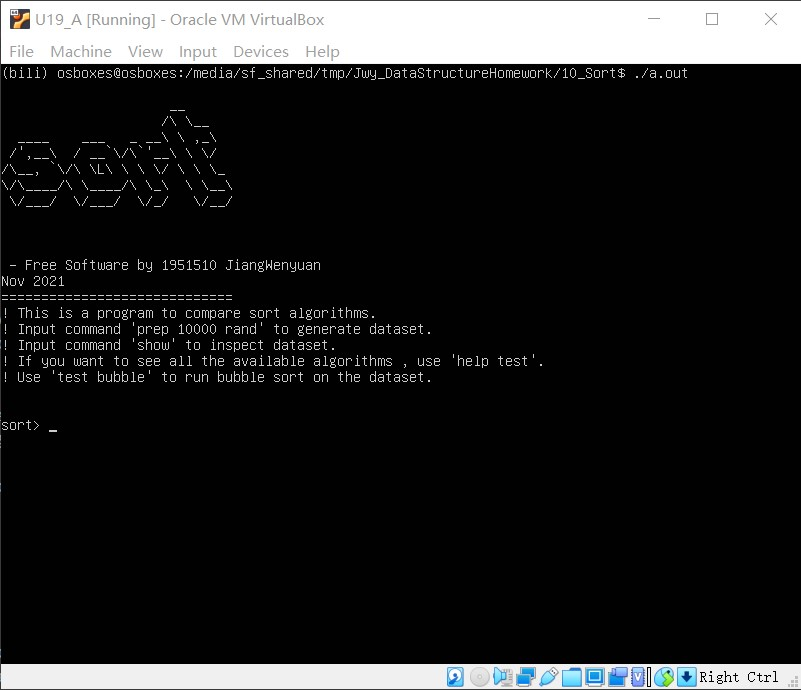
\includegraphics[width=0.7\linewidth]{image/sort_01.jpg}
    \caption{The user interface of the program}
\end{figure}

Usage of commands can be found on the main screen, and the \lstinline{help} command can give you information about theses commands.  All available commands is listed below.

\begin{enumerate}
    \item \lstinline{help} : Show help for a certain command.
    \item \lstinline{exit} : Exit the program.
    \item \lstinline{prep [N] (rand/seq/inv)} : Generate the data for sorting, where \lstinline{[N]} is an integer $> 10$ and $< 1000000$ (the limits depend on your conf and platform).
    \item \lstinline{show} : Show your full dataset.
    \item \lstinline{test (default/bubble/selection/insertion/binsertion/shell/quick/heap/bucket/merge/lsd/msd)} : Run certain sort algorithm and show its performance.
    \item \lstinline{seed} : Show the random seed used in this run.
\end{enumerate}

\subsection{Generate the data for testing sort algorithms}

Type \lstinline{prep 10000 rand} to generate a sequence from 1 to 10000 and randomly suffule them as our dataset for sorting.

\begin{figure}[H]
    \centering
    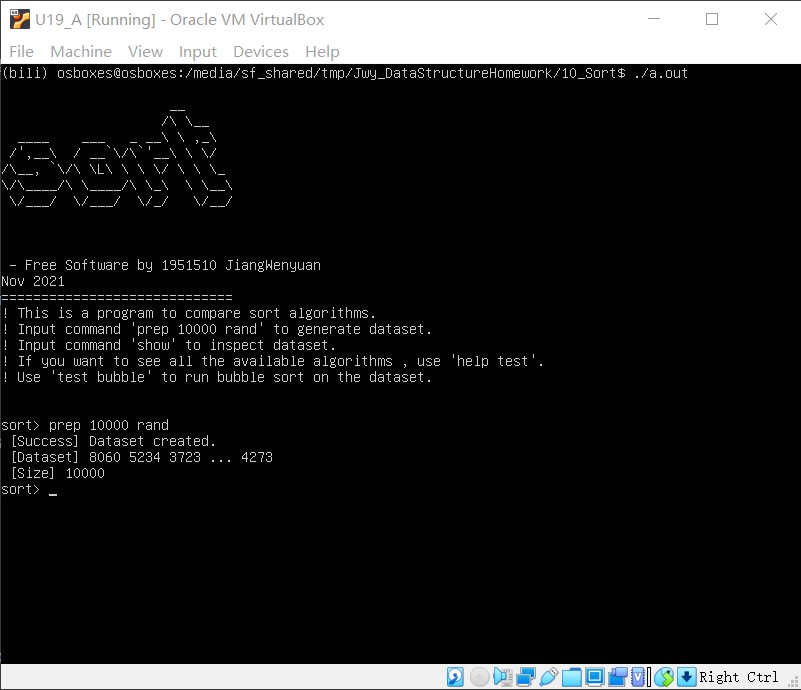
\includegraphics[width=0.7\linewidth]{image/sort_02.jpg}
    \caption{Use \lstinline{prep 10000 rand} to generate dataset (seed: \lstinline{1636865632})}
\end{figure}

To examine our dataset, use \lstinline{show}.

\begin{figure}[H]
    \centering
    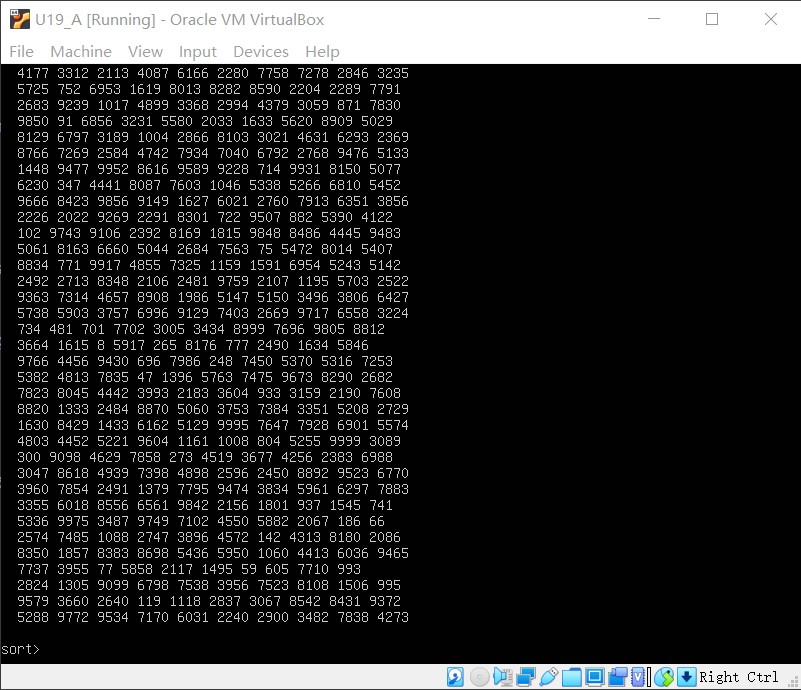
\includegraphics[width=0.7\linewidth]{image/sort_03.jpg}
    \caption{Use \lstinline{show} to view our dataset}
\end{figure}

\subsection{Run an algorithm}

Type \lstinline{test merge} to run Merge Sort on the generated dataset, the results and the performance indicators (Compare func calls, Swap calls and clocks used) will be shown.

\begin{figure}[H]
    \centering
    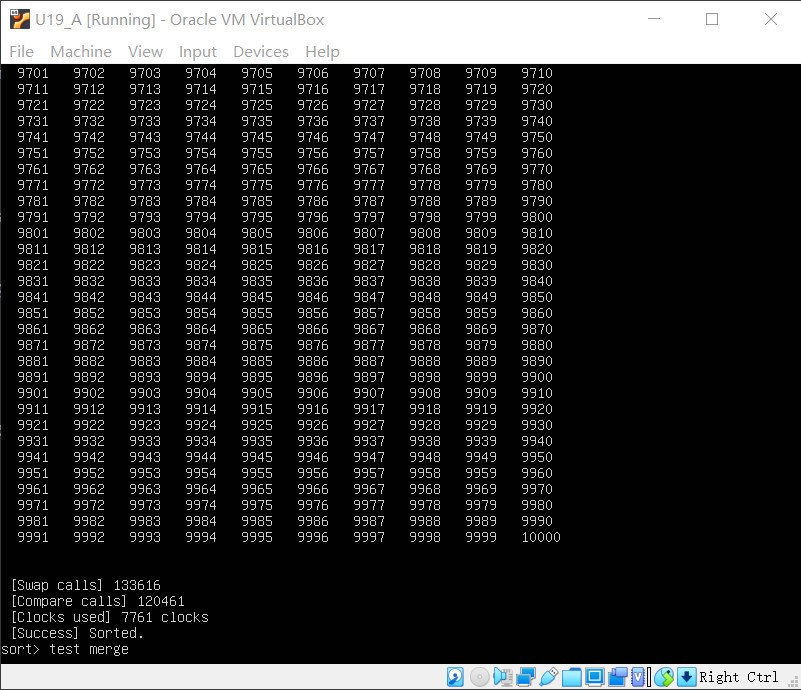
\includegraphics[width=0.7\linewidth]{image/sort_04.jpg}
    \caption{Use \lstinline{test} to run a sort}
\end{figure}

\section{About the Prim's algorithm}

The prim algorithm consists of three major steps:
\begin{enumerate}
    \item Initialize a tree with a given vertex
    \item Expand the tree by one edge: find the minimum-weight edge in the edges that connect the tree to vertices but are not in the tree, and add it to the tree.
    \item Repeat step 2 until all vertices are in the tree.
\end{enumerate}

The pseudocode below demostrats the procedure in more detail.
\begin{algorithm}[H]
    \caption{Prim algorithm}
    \label{alg1}
    \begin{algorithmic}
        \REQUIRE Graph $G$, Starting vertex $a$
        \ENSURE A set $T$, with edges of the minimum spanning tree of $G$
        \STATE \textbf{Initialization:} $T=\{ \varnothing  \}$, $A = \{a\}$.
        \WHILE{$V - A \neq \varnothing$}
        \STATE $S \gets \{ e\,:\, e \notin T, V(e) \cap A \neq \varnothing \}$
        \STATE $e \gets e:\min{C[e]}$
        \STATE Add $e$ to $T$
        \STATE Add $V(e) - (V(e) \cap A)$ to $A$
        \ENDWHILE
        \STATE \textbf{return:} $T$
    \end{algorithmic}
\end{algorithm}

Depending on the data structures used for the graph and the algorithm for finding the minimal edges by weight, the computational complexity can range from $O(n^2)$ to $O(m\, log\, n)$. Using adjacency list to store the graph and a heap (priority queue) to find the most suitable edge is the optimal, which means it can achieve the $O(m\, log\, n)$ complexity.

\section{Notes on the source code}

If you want to modify or re-use the author's code, here are some explaination about the important part of the code. Comments in the source file can pprovide detailed help, but the following shows the outline.

In the author's source code \lstinline{main_header.h}, you can find a line like this in the \lstinline{enetwork} class:
\begin{lstlisting}[language = C++]
map<string, map<string, int>> M;
\end{lstlisting}
The \lstinline{map<string, map<string, int>>} is used to store the graph, which performs even better than adjacency list. The first \lstinline{string} is the source node name, and the second \lstinline{string} is the target node name, with the \lstinline{int} indicating the cost.

Then in the method \lstinline{run_prim(string start_node)}, the set $A$ and $T$ in the pseudocode above is initialized in the following code.
\begin{lstlisting}[language = C++]
    set<string> in_tree;
    vector<edge> ans;
\end{lstlisting}

The code below is the main loop of the prim algorithm, which is exactly the implementation of the pseudocode:
\begin{lstlisting}[language = C++]
    ...
    while (in_tree.size() < M.size())
    {
        priority_queue<edge> q;
        for (auto node : in_tree)
        {
            for (auto node2 : M[node])
            {
                if (in_tree.find(node2.first) == in_tree.end())
                {
                    edge tmp_e;
                    tmp_e.a = node;
                    tmp_e.b = node2.first;
                    tmp_e.cost = node2.second;
                    q.push(tmp_e);
                };
            };
        };
        in_tree.insert(q.top().b);
        ans.push_back(q.top());
    };
    ...
\end{lstlisting}

Detailed implementation of other methods used to maintain the graph data structure follows the textbooks used in this course, and the code may help you understand how each algorithm actually works. Most of the code in \lstinline{main.cpp} and \lstinline{main_header.h} is for processing the user's input, which is not so interesting.

\section{Discussion}

\bibliography{references}
\end{document}
